\section{Calibration and component evidence}
\label{sec:calibration}
\paragraph{Accuracy and calibration improve together.}
Expected calibration error (ECE) compares predicted probabilities with response frequencies in ten equal-width bins, weighted by response count~\citep{paiec2026}. In the formative feedback, pair macro ECE falls from 0.276844 at zero labels to 0.064634 at 31 labels, a 76.65\% reduction. Its budget-weighted macro value is approximately 0.159763.

\begin{figure}[H]
\centering
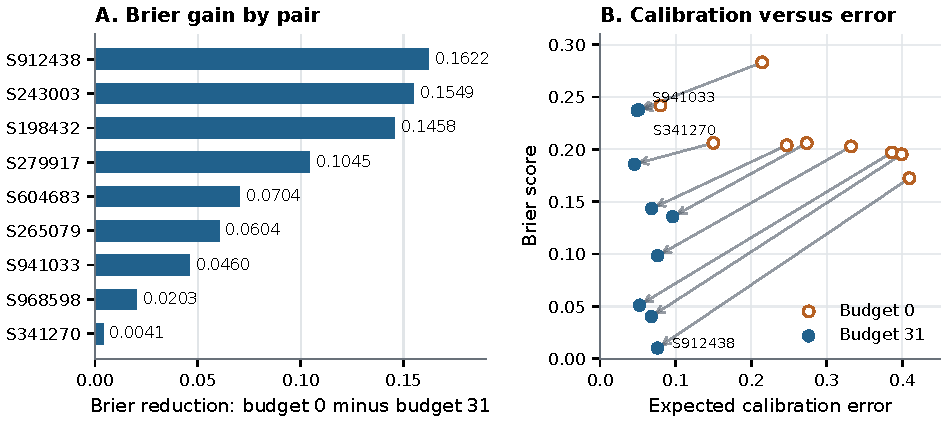
\includegraphics[width=.96\linewidth]{figures/adaptation_calibration.pdf}
\caption{Two complementary views of the formative run. Left: absolute Brier improvement from zero to 31 labels. Right: arrows connect each pair's initial and final ECE--Brier coordinates. Each pair improves in endpoint Brier error; the joint view shows how probability accuracy and calibration change together.}
\label{fig:calibration}
\end{figure}

The two measures also help identify the next modeling opportunity. For S941033, ECE at fifteen labels is 0.015630 while Brier error is 0.237347. Matching an overall response frequency can still leave room to distinguish easier and harder items. We therefore use Brier error as the primary measure and ECE as a complementary diagnostic.

\paragraph{A common-panel component comparison.}
An archived replay evaluated the exact candidate on 153 subject--benchmark pairs across 30 public benchmarks and 21,788 evaluation response rows. The protocol uses the same item split, acquisition stream, and evaluation set across packages~\citep{release}. Table~\ref{tab:local} isolates the recorded results for the Rasch branch, CAIMIRA-style branch, and equal blend.

\begin{table}[H]
\centering
\caption{Archived component replay; lower is better. Three sources (25 pairs) also occur in CAIMIRA training.}
\label{tab:local}
\small
\begin{tabular}{@{}lrrr@{}}
\toprule
Package & Brier ALC & ECE ALC & Brier difference vs. Rasch \\
\midrule
Rasch offset (16) & 0.200183 & 0.150166 & 0.000000 \\
Equal blend (18) & 0.201449 & 0.153118 & +0.001267 \\
CAIMIRA-style native (27) & 0.202985 & 0.156827 & +0.002803 \\
\bottomrule
\end{tabular}
\end{table}

The blend improves on CAIMIRA alone by 0.001536 ALC and on the mean component loss by 0.000135, consistent with Equation~\ref{eq:mixture}. Rasch alone has the strongest point estimate, leading the blend by 0.001267. The two views of adaptation are therefore close in this replay, with equal averaging providing a transparent combination and learned weighting offering a focused next step.

\paragraph{Evidence scope and limitations.}
The formative evaluation establishes a within-run adaptation gain. The local replay uses one seed and label-informed pair selection; 25 pairs share sources with CAIMIRA training. It serves as a component diagnostic. Appendix~\ref{app:training} documents the 44-benchmark CAIMIRA fit; the exact Rasch fitting receipt remains \textbf{UNVERIFIED}. Source-separated comparisons would assess transfer more directly. Appendix~\ref{app:reproduction} describes fresh CPU execution and reproduction.
